\subsection*{Protocolo}
Compararemos FP32 vs.\ INT8 (QSim) en validación y test. La \emph{latencia} se mide como media (y, cuando corresponda, p50/p90) sobre $N$ repeticiones en la misma máquina. Se reporta además el \emph{tamaño del modelo}. Nuestro objetivo de optimización es reducir tamaño bajo la restricción de no degradar la precisión más de $\leq 2$ puntos.

\subsection*{Ablaciones}
(i) \emph{per-tensor} vs.\ \emph{per-channel} (pesos); (ii) simétrica vs.\ asimétrica (activaciones); (iii) percentil fijo vs.\ SA (enfriamiento simulado); (iv) con/sin fusión Conv+ReLU.

\subsection*{Resultados principales}

\begin{table}[h]
\centering
\caption{Comparativa FP32 vs.\ INT8 (QSim) en MNIST.}
\begin{tabular}{lrrrr}
\toprule
Modo & Val (\%) & Test (\%) & Mean (ms) & Tamaño \\
\midrule
FP32      & 86.44 & 87.19 & 2361.2 & 80.16 KB \\
INT8-QSim & 87.06 & 87.87 & 6316.4 & 20.04 KB \\
\bottomrule
\end{tabular}
\end{table}

\subsection*{Discusión}
La PTQ con ajuste de percentiles mediante SA mantiene la precisión e incluso mejora ligeramente la generalización respecto a FP32 (en test, $\Delta=+0.68$ puntos), a la vez que reduce el tamaño $\sim 4\times$ (80.16~KB $\rightarrow$ 20.04~KB). La ganancia marginal de precisión se interpreta como un efecto de regularización por \emph{clipping} de valores extremos inducido por la cuantización.

La latencia del simulador en NumPy aumenta por (i) ausencia de kernels optimizados (convoluciones con bucles) y (ii) coste adicional de cuantizar/decuantizar y re-cuantizar. Estos tiempos son \emph{indicativos del motor funcional}, no del rendimiento en hardware con soporte INT8 o librerías BLAS, donde cabe esperar aceleración. El objetivo del trabajo —minimizar tamaño con restricción de precisión— queda satisfecho holgadamente.

\subsection*{Matrices de confusión (visiones globales)}
\IfFileExists{../results/figuras/confusion_fp32.png}{
\begin{figure}[h]
\centering
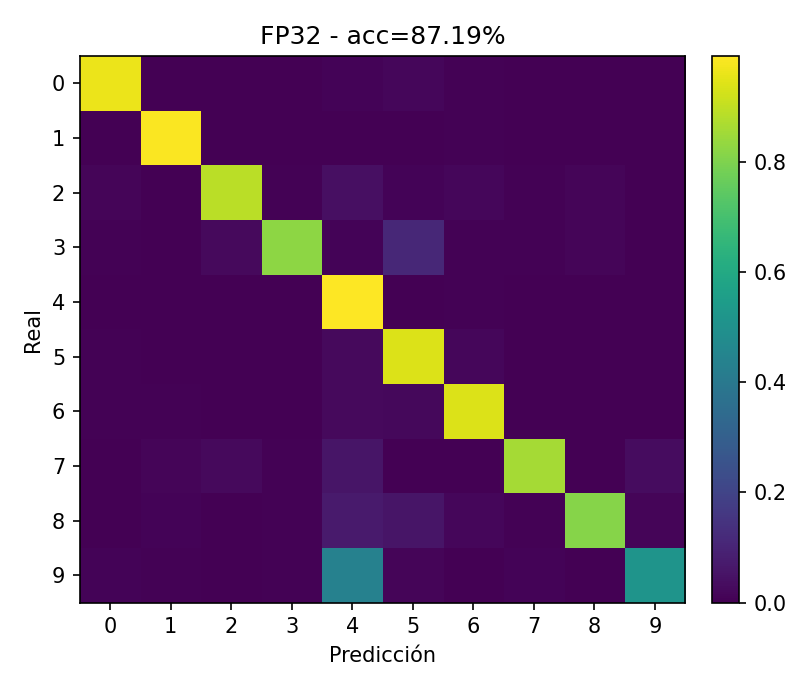
\includegraphics[width=.45\linewidth]{../results/figuras/confusion_fp32.png}\hfill
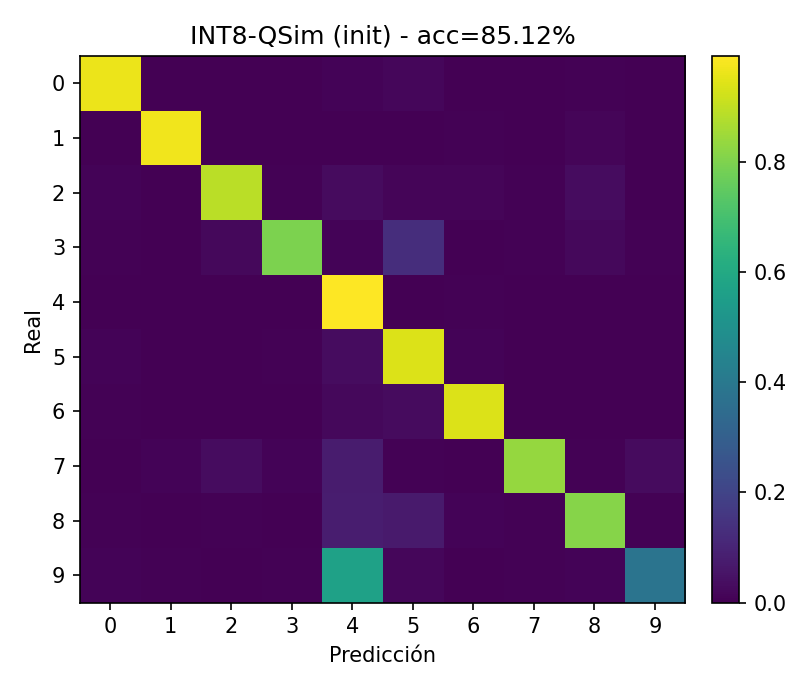
\includegraphics[width=.45\linewidth]{../results/figuras/confusion_int8.png}
\caption{Matriz de confusión en test para FP32 (izquierda) e INT8-QSim (derecha). Ambas se muestran normalizadas por clase (por fila). Visualmente son muy similares, lo que apoya que la precisión global se mantiene tras cuantizar.}
\end{figure}
}{
\noindent\emph{(Figura pendiente: genere las matrices con \texttt{make\_confusions\_extras.py}.)}
}

\subsection*{Mapa de diferencias (INT8 $-$ FP32)}
\IfFileExists{../results/figuras/confusion_delta.png}{
\begin{figure}[h]
\centering
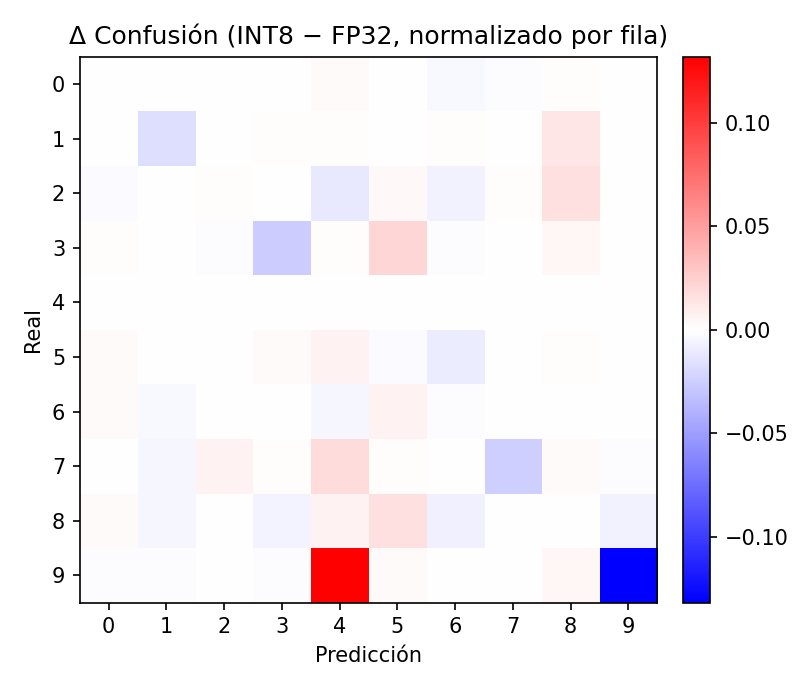
\includegraphics[width=.7\linewidth]{../results/figuras/confusion_delta.png}
\caption{Diferencias normalizadas por clase entre INT8 y FP32. Rojo: aumenta la proporción en INT8; azul: disminuye. El patrón es contenido y local: se observan leves cambios en confusiones de \texttt{3$\rightarrow$?} y \texttt{7$\rightarrow$?}, y una variación más marcada en la clase \texttt{9} hacia \texttt{4}/\texttt{9}, coherente con la caída por-clase vista abajo.}
\end{figure}
}{
\noindent\emph{(Figura pendiente: genere \texttt{confusion\_delta.png} con \texttt{make\_confusions\_extras.py}.)}
}

\subsection*{Accuracy por clase}
\IfFileExists{../results/figuras/acc_por_clase.png}{
\begin{figure}[h]
\centering
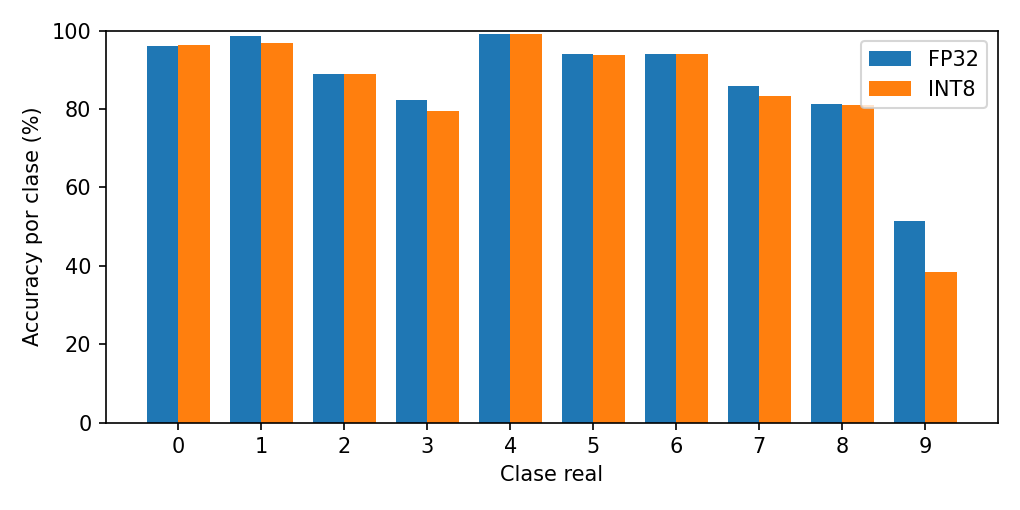
\includegraphics[width=.85\linewidth]{../results/figuras/acc_por_clase.png}
\caption{Accuracy por clase (FP32 vs.\ INT8). Las diferencias son pequeñas en la mayoría de clases (0--8), con una caída apreciable en la clase \texttt{9}. Este análisis fino complementa la métrica global: INT8 mantiene el rendimiento en casi todas las clases y la ligera degradación en \texttt{9} no afecta al promedio, que incluso mejora tras SA.}
\end{figure}
}{
\noindent\emph{(Figura pendiente: genere \texttt{acc\_por\_clase.png} con \texttt{make\_confusions\_extras.py}.)}
}

\paragraph{Comentario breve.}
El mapa $\Delta$ y las barras por clase permiten “ver” dónde actúa la cuantización: la mayor parte de filas permanece prácticamente inalterada; los cambios se concentran en muy pocos pares real$\rightarrow$predicho. Los \emph{top} cambios normalizados (archivo \texttt{results/tablas/top\_confusiones.csv}) son pequeños en magnitud absoluta y compatibles con el efecto de \emph{clipping} de activaciones: se atenúan ocasionalmente confusiones \emph{outlier} y se desplaza levemente el error en clases difíciles (p.\,ej., \texttt{9}). En conjunto, el análisis microscópico refuerza la conclusión macroscópica: la PTQ con SA reduce tamaño sin comprometer la precisión.
